
\documentclass{jarticle}

\setlength{\topmargin}{-45pt}
\setlength{\oddsidemargin}{-7.5mm}
\setlength{\textheight}{24.1cm}
\setlength{\textwidth}{17.4cm}
\setlength{\columnsep}{11mm}

\kanjiskip=.07zw plus.5pt minus.5pt

\usepackage[dvipdfm]{graphicx}
\usepackage{subcaption}
\usepackage{amsmath}
\usepackage{amssymb}
\usepackage{amsfonts} 
\usepackage{multirow}
\usepackage{here}
\usepackage{url}
\usepackage{bm}

\begin{document}

\twocolumn[
\noindent
\hspace{1em}

令和 7 年 前期研究会発表資料
\hfill
\ \ M2 堀本 隆誠

\vspace{2mm}
\hrule
\begin{center}
{\bf \fontsize{13.2pt}{13.2pt}\selectfont RAG を用いたドメイン特化型 LLM の構築および応用
}
\end{center}
\hrule
\vspace{3mm}
]

\vspace{-3mm}
\section{はじめに}
\vspace{-1mm}

近年, 大規模言語モデル (Large Language Models: LLMs) が自然言語処理分野で急速に発展している. しかし, GPT や Gemini のような汎用モデルであっても, アニメ制作のような特定の専門ドメインにおいては, 最新情報の不足, 専門用語の誤解, 事実に基づかない情報 (ハルシネーション) の生成といった課題が存在する.\par

アニメ制作現場において, 過去の作品のスタッフ情報, 制作技術に関する専門用語, ビジネススキームなど, 多岐にわたる正確な知識が求められる. 制作アシスタントがこれらの情報を迅速かつ正確に得られるシステムは, 生産性の向上に大きく貢献する可能性がある. \par

本研究では, Retrieval-Augmented Generation (RAG) と Fine-Tuning (FT) の技術を組み合わせることにより, 高い信頼性と専門性を持つアニメに特化した質問応答システムを構築し,その有効性を評価することを目的とする. \par

\vspace{-3mm}
\section{要素技術}
\vspace{-1mm}

\subsection{Retrieval-Augmented Generation}
\vspace{-1mm}

Retrieval-Augmented Generation (RAG) \cite{RAG_first} は, LLM によるテキスト生成に外部情報の検索を加えることで LLM の回答精度を向上させる技術である. ユーザーの質問に対し, まず関連情報をデータベースから検索 (Retrieve) し, その情報をコンテキストとして LLM に与えることでより事実に基づいた正確な回答を生成 (Generate) させる. これにより, LLM 単体でのハルシネーションを抑制し, 知識の鮮度を保つことが可能となる.

\vspace{-3mm}
\subsection{LoRA}
\vspace{-1mm}

Low-Rank Adaptation (LoRA) \cite{LoRA} とは, 学習するパラメータ数を削減しつつ Fine-Tuning する手法である. モデルの線形層のパラメータを $D_{in} \times D_{out}$ 次元の行列 $W$ とし, 入力ベクトルを $x$ とすると, 出力 $h$ は (1) 式で表される.
\begin{equation}
    h = Wx
\end{equation}
LoRA では線形層のパラメータ $W$ と同次元の差分行列 $\Delta W$ を用意し, 出力 $h$ は (2) 式で表される. 学習の際には $W$ を固定し, $\Delta W$ のみを学習する.
\begin{equation}
    h = Wx + \Delta Wx
\end{equation}
この時, ランク $r$ を設定し, $D_{in} \times r$ 次元の行列 $A$, $r \times D_{out}$ 次元の行列 $B$ で, $\Delta W$ は (3) 式で表せる.
\begin{equation}
    \Delta W = AB
\end{equation}
$W$ のパラメータ数は $D_{in} \times D_{out}$ となる一方で $\Delta W$ のパラメータ数は $r(D_{in} + D_{out})$ となり, 一般的に $r$ は $D_{in}$, $D_{out}$ に比べて非常に小さい値であるため, 学習パラメータ数を大きく減らすことができる.

\vspace{-3mm}
\subsection{量子化}
\vspace{-1mm}

大規模なニューラルネットワークや LLM などの膨大なパラメータを持つモデルでは, 演算の際に膨大な数の乗加算を必要とするため演算に時間がかかる. また, 多くのパラメータを保持するために多くのメモリが必要となる. これらの問題を軽減するためのアプローチとして量子化がある. 一般的に LLM の学習や推論では 16 ビット浮動小数点 (FP16) が用いられることが多いが, これを量子化し 4 ビットに変換する. 本研究で採用した QLoRA で用いられる NormalFloat4 (NF4) と呼ばれるデータ型では, FP16 のパラメータを正規分布に基づいて最適に配置された 16 通りの離散値にマッピングする. 量子化により精度は減少するものの消費するメモリ量を大幅に軽減することができる. \par
Quantized Low-Rank Adaption (QLoRA) \cite{QLoRA} では LLM のパラメータの多くが正規分布に従うことを利用した NormalFloat4 という量子化手法により 4 ビット量子化した LLM において効率的に Fine-Tuning できることを示している. 本研究では, 限られた計算資源 (単一 GPU 環境) で 80 億パラメータを持つ大規模モデルの Fine-Tuning を実現するため, この QLoRA の手法を採用した.

\vspace{-3mm}
\section{提案手法}
\vspace{-1mm}

本研究では, 専門分野の知識を LLM に効果的に統合するため, 複数の検索技術を組み合わせた RAG システムと, 応答品質を向上させるための Fine-Tuning を組み合わせた手法を提案する. \par
LLM は単体では内部知識のみに依存するため, 事実との不整合や情報の陳腐化が課題となる. この課題を解決するために RAG を用いて外部の信頼できる知識源を参照することにより, LLM の回答の事実性と信頼性を担保する. また, 外部情報を Supabase (PostgreSQL) のリレーショナルデータベースに格納する. このような SQL データベースを用いることで, 将来的なデータの追加および更新, 複雑な条件でのデータ抽出が容易になるという利点がある. この外部知識源からユーザーの質問に関連する情報を的確に引き出すために, キーワード抽出 LLM を活用したハイブリッド検索を実装する. \par
まず, ユーザーの質問をキーワード抽出タスクに特化して Fine-Tuning した LLM に入力する. この LLM は, 質問の意図を解析し, 検索に最適化されたキーワードのリストを JSON 形式で生成する. 次に, 生成されたキーワードと元の質問文を使い, 以下の 2 つの検索を並行して実行する.

\begin{itemize}
\item \textbf{全文検索}: 生成されたキーワードを使い, PostgreSQL の N-gram 拡張 (pg\_trgm) を用いて, テキストの一致度が高い外部情報を検索する. これにより, 専門用語や固有名詞を含む外部情報を正確に特定する.
\item \textbf{ベクトル検索}: 元の質問文と外部情報の内容を OpenAI の埋め込みモデル text-embedding-3-small でベクトル化し, それぞれのベクトルの類似度を計算することで類似した外部情報を検索する. これにより, キーワードが直接含まれていなくても文脈的に関連する情報を捉える.
\end{itemize}

これらの検索の比重をそれぞれ 80\%, 20\% とし, 検索結果の上位 5 件を質問応答 LLM に入力する外部情報として扱う. \par
図 \ref{fig:system_diagram} に提案手法のモデル概略図を示す. まず, ユーザーの質問はキーワード抽出 LLM に入力され, 検索キーワードが生成される. 次に, ハイブリッド検索によって外部データベースから最適なコンテキストが抽出される. 最後に, 抽出されたコンテキストと元の質問が応答生成用に Fine-Tuning された質問応答 LLM に入力され, 最終的な回答が生成される.

\begin{figure}[H]
    \centering
    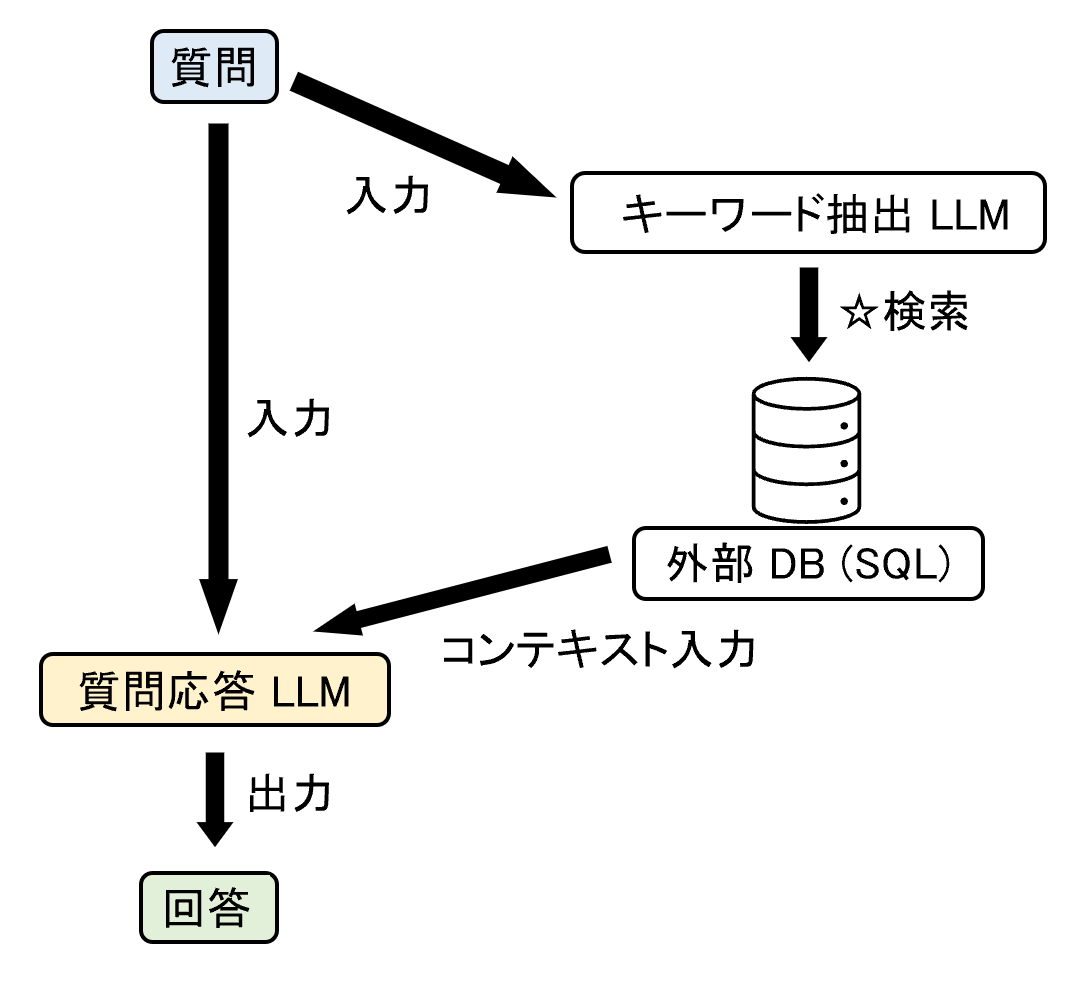
\includegraphics[width=0.8\linewidth]{assets/Figure_system.png}
    \caption{提案システムの全体構成図}
    \label{fig:system_diagram}
\end{figure}

\vspace{-3mm}
\section{実験}
\vspace{-1mm}

提案手法の有効性を検証するため, RAG システムの知識源となる実験データの準備と, LLM の Fine-Tuning および性能比較に関する実験をした. 以下では, 実験データと実験概要について説明する.

\vspace{-3mm}
\subsection{実験データ}
\vspace{-1mm}

本研究における RAG システムの外部知識源として, 以下の 2 種類のデータを統合して使用した.

\begin{itemize}
\item \textbf{AnimeList.csv}: アニメ作品の基本的なメタデータ(タイトル, 話数, 制作会社, 放送時期など)を含む構造化データセット.
\item \textbf{日本語版 Wikipedia}: 各アニメ作品に関する包括的な解説, あらすじ, 登場人物, 制作背景などが含まれる非構造化テキストデータ.
\end{itemize}

これらのデータを統合し, 検索に適した形式に前処理をした. 具体的には, AnimeList.csv の各アニメ作品に対応する Wikipedia の記事を取得し, その記事本文をそれぞれチャンクに分割した. チャンクサイズは 1000 文字, オーバーラップは 100 文字に設定した. これにより生成されたチャンク群を, Supabase (PostgreSQL) データベースに格納し, 各チャンクにベクトル情報と全文検索用のインデックスを付与した. このデータベースが, RAG における検索対象となる. なお, 本研究では AnimeList.csv のうち, ``BLEACH", ``君に届け", ``らんま 1/2", ``クレヨンしんちゃん", ``ONE PIECE", ``犬夜叉", ``カードキャプターさくら", ``ルパン三世", ``ゲゲゲの鬼太郎", ``幽☆遊☆白書", ``蒼い海のトリスティア", ``臭作", ``ロクでなし魔術講師と禁忌教典", ``8 マン", ``どーもくん", ``ガンスミスキャッツ", ``くまみこ", ``瀬戸の花嫁", ``プリンセスチュチュ", ``ウルトラマニアック" の 20 作品を対象にしている. 

\vspace{-3mm}
\subsection{実験概要}
\vspace{-1mm}

本実験では, 構築した RAG システムと Fine-Tuning 済み LLM の性能を評価した. \par

提案手法の中核をなす 2 種類の LLM を, QLoRA を用いて Fine-Tuning した. ベースモデルには, 日本語性能に定評のある elyza/Llama-3-ELYZA-JP-8B (80 億パラメータ) \cite{Llama-3-ELYZA-JP-8B} を使用した.

\begin{itemize}
\item \textbf{キーワード抽出 LLM}: Gemini 2.5 Pro が作成した 100 件の ``質問と検索キーワードリスト" のペアを教師データとして使用し, ユーザーの質問から最適な検索キーワードを JSON 形式で出力するように学習させた. 表 \ref{tab:dataset_for_keyword_LLM} にデータセットの例を示す. 
\item \textbf{質問応答 LLM}: 本研究で構築した RAG システムを用いて Gemini 2.5 Pro が生成した, 100 件の ``コンテキスト付き質問と理想的な回答" のペアを教師データとして使用し, 外部情報に基づいて専門家らしいスタイルで応答を生成するように学習させた. 表 \ref{tab:dataset_for_QA_LLM} にデータセットの例を示す. 
\end{itemize}

\begin{table}[t]
    \centering
    \caption{キーワード抽出 LLM の教師データセット例}
    \vspace{-3mm}
    \label{tab:dataset_for_keyword_LLM}
    \scalebox{0.80}{
    \begin{tabular}{|c|c|} \hline
        質問 & 検索キーワードリスト \\ \hline \hline
        \begin{tabular}{c}
BLEACH における \\ 死神とはなんですか?  
\end{tabular}
& \begin{tabular}{c}
BLEACH, 死神, \\ 用語, 設定, 魂魄    
\end{tabular} \\ \hline
%         \begin{tabular}{c}
% ONE PIECEの「ワノ国編」で \\ 見られた, 浮世絵のような \\ 大胆な色彩設計や作画スタイルは, \\ どのシリーズディレクターの意向が \\ 強く反映されていますか?
% \end{tabular}
% & \begin{tabular}{c}
% ONE PIECE, \\ ワノ国編, \\ シリーズディレクター, \\ 作画, 色彩設計, 演出
% \end{tabular} \\ \hline
        \begin{tabular}{c}
瀬戸の花嫁はパロディが \\ 多用されていますが, \\ アニメの演出として,  \\ 特にどの監督の影響が \\ 色濃く見られますか?
\end{tabular}
& \begin{tabular}{c}
瀬戸の花嫁, \\ パロディ, 演出, \\ 影響, 監督
\end{tabular} \\ \hline
    \end{tabular}
    }
\end{table}

\begin{table}[t]
    \centering
    \caption{質問応答 LLM の教師データセット例}
    \vspace{-3mm}
    \label{tab:dataset_for_QA_LLM}
    \scalebox{0.80}{
    \begin{tabular}{|c|c|} \hline
        コンテキスト付き質問 & 回答 \\ \hline \hline
        \begin{tabular}{c}
 参照情報 (BLEACH) \\「ジャンプフェスタ・\\ アニメツアー'04」にて \\ 上映されたオリジナル \\ アニメを経て (中略) \\ 質問: BLEACH における \\ 死神とはなんですか?
\end{tabular}
& \begin{tabular}{c}
BLEACH における \\ 死神とは, 霊的な \\ 存在で, 悪霊(虚)と \\ 戦い, 魂を \\ 護る存在です. \\ 彼らは尸魂界 \\(ソウルソサエティ)\\ という (以下略)
\end{tabular} \\ \hline
        \begin{tabular}{c}
 参照情報 (ルパン三世) \\ 2010年2月 - \\ テレビスペシャル第21作 \\『ルパン三世 (中略) \\ 質問:
『LUPIN the Third \\ -峰不二子という女-』は, \\ どのような点で革新的な \\ 作品でしたか?
\end{tabular}
& \begin{tabular}{c}
『LUPIN the Third - \\ 峰不二子という女-』は, \\ 従来のルパン三世シリーズと \\ 比べて以下の点で\\ 革新的な作品でした. \\ 1. 監督と制作体制: \\ 従来シリーズとは (以下略)
\end{tabular} \\ \hline
    \end{tabular}
    }
\end{table}

表 \ref{tab:sft_params} に QLoRA のパラメータとして設定した値を示す. \par

\begin{table}[t]
    \centering
    \caption{主要ハイパーパラメータ}
    \vspace{-3mm}
    \label{tab:sft_params}
    \begin{tabular}{|l|c|} \hline
        \textbf{パラメータ名} & \textbf{値} \\ \hline \hline
        LoRA r (ランク) & 8 \\ \hline
        LoRA alpha & 16 \\ \hline
        学習対象の線形層 & モデル内の全線形層 \\ \hline
        Epoch 数 & 20 \\ \hline
        最適化手法 & Paged AdamW (8-bit) \\ \hline
        初期学習率 & 2e-4 \\ \hline
        学習率スケジューラ & linear \\ \hline
    \end{tabular}
\end{table}

 Fine-Tuning の効果と RAG の有効性を検証するため, 以下の 3 つのモデルを用意し, その応答品質を比較した. 

\begin{itemize}
    \item \textbf{モデル A}: RAG + FT 前の ELYZA-JP-8B
    \item \textbf{モデル B}: RAG + FT 後の ELYZA-JP-8B 
    \item \textbf{モデル C}: Gemini 2.5 Pro
\end{itemize}

\vspace{-3mm}
\section{実験結果}
\vspace{-1mm}

テスト用データとして 20 作品に対してそれぞれ 1 つずつの計 20 個の質問を用意した. その結果として, 20 問中 1 問のみ正答が得られた. そこで, その質問文 ``ルパン三世のモンキーパンチが最後に書いた漫画はなんですか?" を入力した結果を示す. このとき, キーワード抽出 LLM により, ``ルパン三世, モンキーパンチ, 最後の漫画, ルパン, パンチ" というキーワードが得られた. キーワード検索をすることで求める答えがある情報をもつ記事にヒットしやすいキーワードである ``モンキーパンチ, 最後の漫画" が得られた一方, ``ルパン, パンチ" のようにキーワードとしてはあまり意味をなさない単語が抽出されていることがわかった. これは, 本質問とはそのキーワード単体では関係のない単語であるが, 一般的な言葉として使われている単語のため抽出されてしまったと考えられる. 表 \ref{tab:results} に 3 つのモデルの質問に対するそれぞれの回答を示す.

\begin{table}[t]
    \centering
    \caption{各モデルによる回答の品質比較}
    \vspace{-3mm}
    \label{tab:results}
    \scalebox{0.80}{
    \begin{tabular}{|c|c|} \hline
        質問文 & \begin{tabular}{c}
ルパン三世のモンキーパンチが \\ 最後に書いた漫画はなんですか?
\end{tabular}\\ \hline \hline
        モデル & 生成された回答 \\ \hline
        A & \begin{tabular}{c}
モンキー・パンチが最後に書いた漫画は, \\ 1994 年イタリアの雑誌「Kappa Magazine 22」\\ に掲載された『\textbf{ルパン三世・ALIS PLAUD}』です. 
\end{tabular}\\ \hline
        B & \begin{tabular}{c}
イタリアの雑誌「Kappa Magazine 22」に \\ 掲載された『\textbf{ルパン三世・ALIS PLAUD}』です. \\ これは単体作品としてはモンキー・パンチ \\ 自身による最後の作品となります. \\ ただし, モンキー・パンチは『漫画アクション』 \\ 1994 年 8 月 26 日号に掲載された \\ 「ルパン三世対斬鉄剣」の作画監修も行っています.  \\ これは『ルパン三世 燃えよ斬鉄剣』の \\ 前日談を描いた作品です. 
\end{tabular} \\ \hline
        C & \begin{tabular}{c}
モンキー・パンチ先生が最後に完全な新作として \\ 発表した連載漫画は, 『M.F.C. 女泥棒会社』\\(1982 年 - 1983 年)とされています. \\(以下略)
\end{tabular} \\ \hline
    \end{tabular}
    }
\end{table}

質問文 ``ルパン三世のモンキーパンチが最後に書いた漫画はなんですか?" に対する正解の漫画は ``ルパン三世・ALIS PLAUD" である. モデル A は正解を正確に述べているが, 単純な回答になっている. 一方, モデル B はより背景知識を補い, 詳細な回答を生成している. これは,  Fine-Tuning によって情報の統合能力と応答スタイルが改善されたことを示唆していると考えられる. モデル C では, 高い知識を持っていたが, 回答した漫画のタイトルが間違っていた. 回答した漫画のタイトル ``M.F.C. 女泥棒会社" は, ``ルパン三世" のスピンオフ作品ではあるが, モンキー・パンチが描いたのではなく, 鈴木イゾという漫画家が描いたものである. これらの結果から, RAG による事実性の担保と, FT による専門性の付与を組み合わせた提案手法の有効性が確認された. 今後は正解数を増やすとともに定量的な評価を目指す. 


\vspace{-3mm}
\section{まとめと今後の課題}
\vspace{-1mm}

本研究では, アニメ制作の専門分野に特化した高信頼な質問応答システムを構築するため, RAG と Fine-Tuning を組み合わせた手法を提案した. 具体的には, AnimeList.csv と Wikipedia から作成した外部知識をデータベースに保存し, キーワード抽出 LLM を用いたハイブリッド検索によって高精度な情報検索を実現する RAG システムを構築した. さらに, このシステムを用いて生成した高品質な Q\&A データセットで LLM を Fine-Tuning することにより, 応答の専門性と品質を向上させた. 比較実験の結果, RAG を用いないモデルが専門的な質問に回答できない一方で, 提案手法である RAG と Fine-Tuning を組み合わせたモデルは, 単純な RAG のみのモデルと比較して, より文脈を深く理解し, 専門家らしい流暢で付加価値の高い回答を生成できることが示された. このことから, 提案手法がドメイン特化型 AI の構築において有効であることが確認された. \par

今後の課題としては, まず Fine-Tuning 用データセットの規模を数百から数千件へと拡充し, モデルのさらなる性能向上を目指す必要がある. また, 現在は単一の検索および生成プロセスであるが, 質問の意図に応じて検索戦略を自律的に変更したり, 複数の情報源を段階的に参照したりする, より高度な RAG アーキテクチャの実装が望まれる. 加えて, 本研究での評価は主に人手による定性的なものであったため, 定量的評価により性能を客観的に示すことも重要な課題である. これらの課題に取り組むことで, 将来的には制作現場の多様なニーズに応える, より実践的な AI アシスタントの実現が期待される.

\vspace{-3mm}
\bibliography{index}
\bibliographystyle{junsrt}

\end{document}
